% Main manuscript: compile main.tex with pdfLaTeX and BibTeX.
% Required template files: sn-jnl.cls and sn-mathphys-num.bst.
%%%%%%%%%%%%%%%%%%%%%%%%%%%%%%%%%%%%%%%%%%%%%%%%%%%%%%%%%%%%%%%%%%%%%%

\documentclass[pdflatex,sn-mathphys-num]{sn-jnl}

\usepackage{graphicx}%
\usepackage{multirow}%
\usepackage{amsmath,amssymb,amsfonts}%
\usepackage{amsthm}%
\usepackage{mathrsfs}%
\usepackage{xcolor}%
\usepackage{textcomp}%
\usepackage{manyfoot}%
\usepackage{booktabs}%
\usepackage{listings}%
\usepackage{tabularx}%
\usepackage{array}%
\usepackage{makecell}%
\usepackage{adjustbox}%
\usepackage{enumitem}%
\usepackage{tikz}%
\usepackage{pgfplots}%
\usetikzlibrary{arrows.meta,positioning,fit,backgrounds,calc}
\pgfplotsset{compat=1.18}
\usepgfplotslibrary{groupplots}

\theoremstyle{thmstyleone}%
\newtheorem{theorem}{Theorem}%
\newtheorem{proposition}[theorem]{Proposition}%
\theoremstyle{thmstyletwo}%
\newtheorem{example}{Example}%
\newtheorem{remark}{Remark}%
\theoremstyle{thmstylethree}%
\newtheorem{definition}{Definition}%

\raggedbottom

\begin{document}

\title[Cognitive-Task-Aware RAG for Cyber Threat Intelligence]{Cognitive-Task-Aware Retrieval-Augmented Generation for Cyber Threat Intelligence}

\author*[1]{\fnm{First} \sur{Author}}\email{first.author@example.edu}

\author[1]{\fnm{Second} \sur{Author}}\email{second.author@example.edu}

\author[2]{\fnm{Third} \sur{Author}}\email{third.author@example.edu}

\affil*[1]{\orgdiv{Department of Computer Science}, \orgname{University Name}, \orgaddress{\city{City}, \country{Country}}}

\affil[2]{\orgdiv{Department}, \orgname{Institution Name}, \orgaddress{\city{City}, \country{Country}}}


\abstract{Cyber threat intelligence (CTI) assistants must produce heterogeneous outputs, including categorical answers, weakness identifiers, severity vectors, and technique sets. We introduce Cognitive-Task-Aware Retrieval-Augmented Generation (CTA-RAG), which routes unlabelled requests to specialist retrieval, prompting, and parsing pipelines. We evaluate seven configurations on four CTIBench tasks with a common configured answer model. CTA-RAG achieves 74.84\% multiple-choice accuracy, 73.40\% weakness-mapping accuracy, severity mean absolute difference of 1.0990, and mean per-instance technique-extraction F1 of 0.9554. Relative to Unified RAG, weakness accuracy increases by 4.70 percentage points and severity error decreases by 0.1648; both contrasts remain different after Holm correction across 24 comparisons, although the severity result is close to the 0.05 threshold. Adaptive-RAG-adapted has the highest multiple-choice accuracy, and CTA-RAG's additional technique-extraction gain over Unified RAG is not resolved by the adjusted test. Automatic routing is correct on 4,550 of 4,560 main-run items ; robustness to instruction rewrites is not established by these runs. Paired analysis shows that retrieval configurations both rescue and damage decisions. External evaluation supports weakness mapping on 290 CTIConnect items, without establishing transfer for the other tasks. These findings support task specialization for selected output contracts while distinguishing predictive quality, routing robustness, and operational reliability.}

\keywords{Cyber threat intelligence, Retrieval-augmented generation, Large language models, Task routing, MITRE ATT\&CK, CVSS, Security operations}

\maketitle

\section{Introduction}\label{sec:intro}

Consider a typical hour in a security operations centre. An analyst may need to determine which ATT\&CK tactic corresponds to a described adversary behaviour, assign the primary Common Weakness Enumeration (CWE) identifier to a newly disclosed vulnerability, derive its CVSS severity vector for patch prioritisation, extract all relevant ATT\&CK techniques from an incident report, and attribute an intrusion to a likely threat actor. Although these requests arrive through the same analyst workflow, they are fundamentally different computational tasks: factual recall, taxonomic mapping, rule-based scoring, structured extraction, and evidence-driven attribution. Growing scale and complexity of cyber operations make automating such workflows increasingly important. Cyber threat intelligence (CTI) is therefore becoming not only more important but increasingly dependent on systems capable of transforming large volumes of heterogeneous security information into reliable, machine-consumable intelligence.

Large language models (LLMs) are natural candidates for this role. They can interpret technical security narratives, identify attack patterns, extract structured information, and synthesize evidence across lengthy reports. Recent surveys identify generative AI as a rapidly expanding area of cybersecurity research \citep{ferrag2024generative,xu2024llm4sec}, while operational systems have demonstrated the extraction of structured STIX objects from unstructured threat reports \citep{siracusano2023action}, mapping of narrative descriptions to ATT\&CK tactics \citep{fayyazi2023uses}, and automated coding of CTI variables from cybercrime-forum content \citep{clairoux2024llm}. CTIBench \citep{alam2024ctibench} further consolidated these capabilities into a multi-task benchmark, demonstrating that general-purpose LLMs such as GPT-4 can address diverse CTI tasks without task-specific training. However, the ability to generate an answer does not imply that the answer is sufficiently reliable for operational use. Three limitations are particularly consequential in CTI. First, \emph{parametric knowledge becomes stale}: model knowledge is bounded by training data, whereas resources such as the National Vulnerability Database, CWE, and MITRE ATT\&CK continuously introduce and revise vulnerabilities, weaknesses, techniques, and relationships \citep{nvd2024,mitre2024cwe,mitre2024attack}. Second, \emph{structured security identifiers are vulnerable to hallucination}: an LLM can produce a syntactically valid \texttt{CWE-787}, CVSS vector, or \texttt{T1055} while assigning it to the wrong vulnerability or behaviour \citep{ferrag2024generative,alam2024ctibench}. Such errors are particularly problematic because authoritative-looking identifiers can propagate directly into ticketing, prioritisation, detection, and reporting workflows. Third, \emph{analytical inference remains brittle}: tasks such as distinguishing process injection from broader defence-evasion behaviour or attributing an intrusion from multiple weak signals require evidence composition rather than surface-level semantic matching. These limitations motivate grounding LLM-based CTI systems in external, current, and task-relevant evidence—but, as we show, grounding alone is not sufficient.


Retrieval-augmented generation (RAG) offers a natural response to these limitations by grounding generation in evidence retrieved at inference time \citep{lewis2020rag,karpukhin2020dense,izacard2021fid}. In cybersecurity, RAG has been used to integrate global and organisation-specific threat knowledge \citep{mitra2024localintel}, improve ATT\&CK interpretation over ungrounded prompting \citep{fayyazi2024ttp}, and maintain access to emerging vulnerabilities and attack patterns \citep{borah2025adapting}. However, grounding alone does not resolve the heterogeneity of CTI workflows. The five tasks described above require not only different evidence, but fundamentally different output contracts: a categorical choice, an exact identifier such as \texttt{CWE-79}, a complete \texttt{CVSS:3.1} vector, a set of ATT\&CK technique identifiers, or a named threat actor.

This heterogeneity exposes a fundamental limitation of conventional RAG. A unified retrieve–generate pipeline assumes that the same retrieval strategy, prompt structure, decoding configuration, and output handling are suitable across tasks. Such an assumption is reasonable for homogeneous question answering but problematic for CTI, where factual retrieval, hierarchical classification, algorithmic scoring, multi-label extraction, and attribution impose different requirements \citep{alam2024ctibench,shi2023distracted,jeong2024adaptive,asai2023selfrag}. More importantly, additional retrieval is not necessarily beneficial. In weakness mapping, for example, semantic retrieval from the CWE taxonomy can return a highly related child or sibling weakness rather than the NVD primary class. The retrieved evidence is relevant and authoritative, yet it can anchor the model to the wrong identifier under exact-match evaluation \citep{nvd2024,mitre2024cwe,shi2023distracted}. Our current paired comparisons show that retrieval-based systems can improve aggregate performance while changing some previously correct decisions to incorrect ones. This observation motivates a broader principle: effective CTI RAG requires deciding not only \emph{what} evidence to retrieve, but also \emph{whether and how} retrieval should be performed and \emph{how the resulting answer should be generated and validated}. Crucially, this decision must precede retrieval; once mismatched evidence enters the context, it can influence subsequent generation.

Recent adaptive RAG methods partially address this problem. Self-RAG determines when retrieval is necessary \citep{asai2023selfrag}; GraphRAG reorganises evidence through graph structure and hierarchical summaries \citep{edge2024graphrag}; Adaptive-RAG adjusts retrieval depth according to estimated query complexity \citep{jeong2024adaptive}; and TAdaRAG introduces intent-driven adaptation for domain-specific extraction \citep{zhang2026tadarag}. These approaches demonstrate that retrieval need not be uniform. However, they primarily adapt evidence acquisition, whereas CTI additionally requires adaptation of the downstream generation and validation process. A prompt designed to derive a complete CVSS vector, for example, is fundamentally different from one intended to identify a primary CWE class, as are the parsers required to validate their outputs. A further gap arises at the routing stage. CTIBench provides each task separately with task-specific instructions \citep{alam2024ctibench}; consequently, task identity is effectively known before inference. This evaluates performance under \emph{labelled task selection}, whereas a deployed CTI assistant receives heterogeneous analyst requests and must first infer what kind of output is required. Pipeline selection is therefore itself part of the problem and should be evaluated independently rather than assumed to be given. These observations expose three gaps in existing CTI RAG systems: \textbf{(i) schema-specific pipeline adaptation}, because heterogeneous output contracts require different retrieval, prompting, decoding, and parsing strategies; \textbf{(ii) automatic task selection}, because real analyst requests do not arrive with oracle pipeline labels; and \textbf{(iii) task-dependent retrieval utility}, because relevant retrieval can improve, have little effect on, or actively degrade performance depending on the requested output.

To address aforementioned challenges, we propose \textbf{Cognitive-Task-Aware Retrieval-Augmented Generation (CTA-RAG)}, an architecture that makes the cognitive and structural requirements of a request an explicit input to pipeline selection. CTA-RAG organises CTI tasks into four cognitive modes—\emph{memorization} for factual recall, \emph{understanding} for taxonomic interpretation, \emph{problem-solving} for algorithmic scoring, and \emph{reasoning} for structured inference and attribution—implemented through five schema-specific modules. Each module owns its retrieval source and depth, prompt architecture, decoding configuration, and output parser. A lightweight cascade router selects the appropriate module directly from the unlabelled query before retrieval, without access to gold answers or oracle task labels. We evaluate CTA-RAG on CTIBench against a locally executed Closed Book control, Unified RAG, and four retrieval-adaptive configurations while controlling the answer generator, supporting comparison of complete configurations without establishing component-level causality.

We ask three research questions: \textbf{RQ1}, does complete task specialization outperform a shared RAG pipeline; \textbf{RQ2}, can the appropriate specialist be selected automatically; and \textbf{RQ3}, when does retrieval help or hurt? Section~\ref{sec:results} answers these questions using paired outcomes, routing diagnostics, and paired system comparisons.

\noindent\textbf{The key contributions of this work are as follows:}
\begin{enumerate}[leftmargin=*,nosep,topsep=2pt]
\item We introduce \textbf{CTA-RAG}, a task-conditional CTI architecture in which four cognitive modes are realised through five schema-specific pipelines that jointly adapt retrieval, prompting, decoding, and output parsing.

\item We develop an \textbf{oracle-free cascade router} that selects the appropriate pipeline directly from an unlabelled analyst query before retrieval, making routing accuracy a separately measurable component of end-to-end performance.

\item We conduct a \textbf{controlled evaluation on CTIBench} against a locally executed Closed Book control, Unified RAG, and four retrieval-adaptive configurations under a matched answer generator, with paired statistics and full-attempt denominators; the clearest adjusted advantages over Unified RAG are on weakness mapping and severity prediction.

\item We quantify rescues and damages in paired predictions, showing that end-to-end gains can coexist with item-level regressions without attributing those changes to retrieval alone.

\item We measure automatic routing on the current controlled runs and distinguish route correctness from downstream answer correctness; transfer to unconstrained instructions remains untested.
\end{enumerate}


\section{Related Work}\label{sec:related}

The automation of threat intelligence began long before language models, and it began with vocabulary. Before anything could be reasoned about automatically, the community had to agree on what an adversary technique, an indicator, and a campaign actually were, which produced MITRE ATT\&CK as a shared behavioural taxonomy \cite{mitre2024attack} and STIX/TAXII as the exchange substrate \citep{oasis2021stix,oasis2021taxii}. Around these grew knowledge graphs linking vulnerabilities, actors, and techniques into queryable structure \citep{li2022attackg}, alongside a literature concerned with what threat intelligence is for and how its quality should be judged \citep{tounsi2018survey,schlette2021measuring,mcmillan2013definition}. This work matters to our argument for a reason that is easy to overlook: it established that CTI outputs are \emph{typed}. A weakness class, a severity vector, and a technique identifier are not interchangeable strings but members of distinct, externally governed vocabularies with their own validity conditions. Every subsequent system inherits that constraint whether or not it acknowledges it.

Language models arrived into this structured world and were immediately useful. They summarise vulnerability disclosures, process reports, identify techniques, and extract structured intelligence from prose \citep{ferrag2024generative,xu2024llm4sec}, with concrete systems converting reports into STIX objects \citep{siracusano2023action}, mapping ambiguous attack descriptions onto ATT\&CK tactics \citep{fayyazi2023uses}, and coding intelligence variables from criminal-forum discussion \citep{clairoux2024llm}. The difficulty surfaced quickly and was the same difficulty everywhere: models fluent in the \emph{form} of a CWE identifier or a CVSS vector are not thereby reliable about its \emph{content}, and their knowledge of which CVEs exist decays continuously after training. Fluency in a governed vocabulary without grounding in it is precisely the recipe for confident error.

Retrieval-augmented generation was the natural correction, conditioning generation on documents fetched at inference time \citep{lewis2020rag,karpukhin2020dense,izacard2021fid} and thereby connecting the model to live NVD, CWE, and ATT\&CK content. Security applications followed: LocalIntel fuses global threat repositories with organisation-local knowledge \citep{mitra2024localintel}, and retrieval measurably improves ATT\&CK tactic and technique analysis over direct prompting \citep{fayyazi2024ttp}. Closest to the present work, Borah and colleagues address the staleness problem head-on, building a retrieval framework to keep a model current on emerging vulnerabilities and attack patterns, and showing that a hybrid retrieval strategy outperforms baseline dense retrieval on knowledge retention and temporal reasoning \citep{borah2025adapting}. Their result is important for us in two ways. It confirms that the retrieval \emph{mechanism} is a productive axis of improvement for CTI, and it locates that improvement upstream of the answer: what changes is how evidence is found and how current it is, not what contract the answer must satisfy. Their axis and ours are orthogonal, and we return in Section~\ref{sec:conclusion} to the fact that they compose. The paradigm works. What it left unexamined is the assumption baked into its own name---that generation is one thing to be augmented in one way.

Retrieved content can also carry adversarial instructions: indirect prompt injection places malicious instructions in third-party data consumed by an application \citep{greshake2023injection}. This motivates source isolation and output validation in CTI pipelines, but neither property establishes resistance to semantically valid malicious answers. We evaluate benign inputs and do not claim a measured poisoning or injection defence.

There is also a routing literature, and it is worth distinguishing carefully from ours because the word is
shared and the referent is not. Model routing selects \emph{which model} answers a query, trading quality against
cost by sending easy queries to cheap models and hard ones to frontier models \citep{chen2023frugalgpt,
ding2024hybridllm, ong2024routellm}. That axis is orthogonal to the one we take. A model router asks how much
capability a query deserves; CTA-RAG's router asks what kind of artefact the query demands. The two compose
naturally---a deployment could select the pipeline first and the model within it second---and neither substitutes
for the other, because choosing a larger model does not tell a system to emit an identifier rather than prose.

Broader NLP research then began to question exactly that assumption, though from a particular angle. Self-RAG made retrieval conditional, letting the model judge when external evidence is needed and critique what it receives \citep{asai2023selfrag}. GraphRAG replaced flat passage retrieval with entity graphs and hierarchical community summaries, which pays off on questions requiring global synthesis \citep{edge2024graphrag}. Adaptive-RAG conditioned retrieval depth on estimated query complexity, routing simple questions to cheap paths and hard ones to iterative retrieval \citep{jeong2024adaptive}. TAdaRAG went furthest toward our position, using intent-driven routing to select domain-specific extraction templates and construct task-adapted knowledge structures on the fly \citep{zhang2026tadarag}. Read together, this line of work establishes something important: uniform retrieval is a design choice, not a necessity, and relaxing it helps. But the adaptation in each case terminates at or near the retrieval boundary. Evidence selection, depth, timing, and structure vary; the prompt that consumes the evidence and the parser that validates the output largely do not.

That terminus is defensible in open-domain question answering, where outputs are free-form text and one answer template genuinely suffices. It is not defensible in CTI. The parser that accepts \texttt{CWE-79} rejects a prose explanation of why cross-site scripting applies; the scorer that computes mean absolute deviation over CVSS base scores requires all eight metrics in a parseable vector; multi-label technique F1 requires \texttt{T\#\#\#\#} tokens rather than technique names \citep{alam2024ctibench,mitre2024cwe,first2024cvss,mitre2024attack}. When the output contract is this rigid, adapting retrieval while sharing the answer stack solves the easier half of the problem. Related evidence from outside security supports the concern directly: irrelevant or merely adjacent retrieved context distracts language models and degrades accuracy \citep{shi2023distracted}, motivating the paired decision analysis in Section~\ref{sec:ablations}. Prompting research offers complementary levers, with chain-of-thought and self-consistency improving multi-step inference \citep{wei2022chain,wang2023selfconsistency}, but these are applied to a task, not selected between tasks.

Benchmarking closes the circle and reveals the last gap. CTIBench assembled multiple-choice knowledge, root-cause mapping, vulnerability severity prediction, technique extraction, and threat-actor attribution into one evaluation, and reported strong but uneven zero-shot performance for general-purpose models \citep{alam2024ctibench}. Its structure, however, encodes an assumption worth naming: because each task ships with its own instruction header in its own file, task identity is available before an answer is attempted. Systems are therefore measured on labelled-task solving. The analyst's queue does not arrive labelled. Our work sits precisely in the space these three literatures leave open---typed outputs from the standards tradition, retrieval adaptation from the RAG tradition, and unlabelled multi-task evaluation that the benchmark tradition has not yet demanded---by conditioning retrieval, prompting, decoding, and parsing jointly on an inferred task type, and by scoring that inference separately.

\section{Cognitive-Task-Aware RAG}\label{sec:method}

\subsection{Problem formulation}\label{sec:formulation}

Let $q$ denote an incoming analyst request, comprising an instruction span and a content payload. Conventional RAG computes $A(q)=G(P(q,R(q)))$ with a single retriever $R$, prompt constructor $P$, and generator $G$. CTA-RAG replaces this with a family of pipelines indexed by an inferred task type:
\begin{equation}
A(q)=G_{\hat{\tau}}\!\bigl(P_{\hat{\tau}}(q,R_{\hat{\tau}}(q))\bigr),
\qquad
\hat{\tau}=\textsc{Route}(q),
\label{eq:cta}
\end{equation}
where $\textsc{Route}$ emits a pipeline label, $R_{\hat{\tau}}$ retrieves from a task-matched index with a task-specific depth, $P_{\hat{\tau}}$ constructs a schema-aware prompt, and $G_{\hat{\tau}}$ decodes under task-specific settings into a parser that enforces the output contract. The deployed label space is
\begin{equation}
\begin{aligned}
\hat{\tau} \in \{&
\texttt{memorization},\
\texttt{understanding},\
\texttt{problem\_solving},\\
&
\texttt{reasoning\_ate},\
\texttt{reasoning\_taa}
\}.
\end{aligned}
\label{eq:router-space}
\end{equation}

Two design decisions deserve justification. First, the label space has five elements while the cognitive inventory has four. Technique extraction and threat-actor attribution are both reasoning tasks in the benchmark's own taxonomy \citep{alam2024ctibench}, but they require different retrieval stores (technique descriptions versus intrusion-set profiles), different prompts (enumeration versus hypothesis-driven attribution), and different parsers (identifier sets versus named entities). Collapsing them would force one of the two to use a mismatched contract, so the cognitive grouping informs design while the module inventory follows the schema.

Second, $\hat{\tau}$ is discrete and single-valued. We deliberately do not compute continuous cognitive-demand features at inference and blend pipelines, because the downstream scorers accept mutually exclusive artefacts: a letter, an identifier, a vector, a set, a name. A soft mixture over incompatible contracts has no valid projection into any of them. Cognitive structure therefore enters at design time, shaping each module's index, prompt, and parser according to the reasoning role it serves \citep{newell1972human,anderson1983architecture}, and enters at inference only through a hard selection.

Figure~\ref{fig:arch} shows the resulting flow: one routing decision, one pipeline, one generation.

\begin{figure*}[t]
\centering
\resizebox{\textwidth}{!}{%
\iffalse
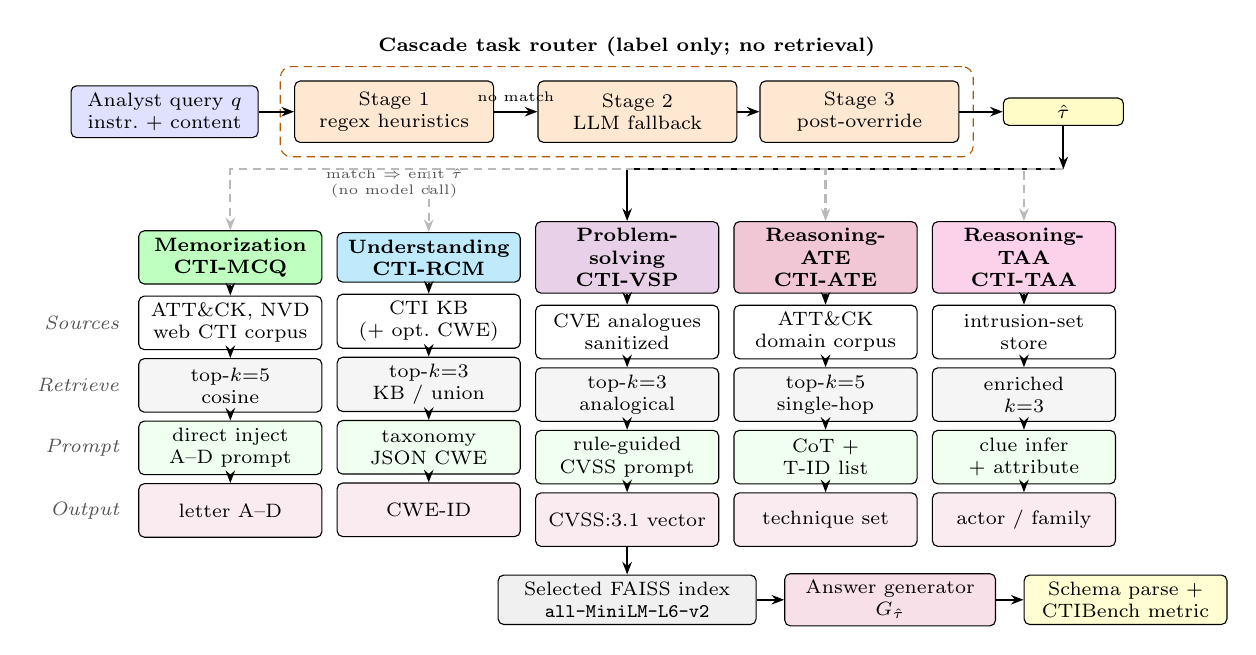
\begin{tikzpicture}[
    font=\scriptsize,
    >=Stealth,
    box/.style={draw, rounded corners=2pt, align=center, inner sep=2.5pt},
    stage/.style={box, fill=white, text width=2.15cm, minimum height=0.68cm},
    head/.style={box, text width=2.15cm, font=\scriptsize\bfseries, minimum height=0.58cm},
    rbox/.style={box, fill=orange!18, text width=2.35cm, minimum height=0.78cm},
    arr/.style={-{Stealth[length=1.6mm]}, thick},
    darr/.style={-{Stealth[length=1.6mm]}, thick, densely dashed, gray!55}
]
\node[box, fill=blue!12, text width=2.2cm] (q)
    {Analyst query $q$\\instr.\ + content};

\node[rbox, right=0.45cm of q] (h) {Stage~1\\regex heuristics};
\node[rbox, right=0.55cm of h] (l) {Stage~2\\LLM fallback};
\node[rbox, right=0.28cm of l] (o) {Stage~3\\post-override};
\node[box, fill=yellow!22, text width=1.35cm, right=0.55cm of o] (tau) {$\hat{\tau}$};

\begin{scope}[on background layer]
  \node[draw=orange!70!black, densely dashed, rounded corners, inner sep=5pt,
        fit=(h)(l)(o),
        label={[font=\scriptsize\bfseries]above:Cascade task router (label only; no retrieval)}] {};
\end{scope}

\draw[arr] (q) -- (h);
\draw[arr] (h) -- (l) node[midway, above, font=\tiny, sloped] {no match};
\draw[arr] (l) -- (o);
\draw[arr] (o) -- (tau);
\node[font=\tiny, gray!65!black, below=0.20cm of h, align=center]
    {match $\Rightarrow$ emit $\hat{\tau}$\\(no model call)};

\coordinate (midtop) at ($(q.west)!0.5!(tau.east)$);
\node[head, fill=green!25] (m0) at ([xshift=-4.66cm,yshift=-1.85cm]midtop)
    {Memorization\\CTI-MCQ};
\node[head, fill=cyan!25, right=0.18cm of m0] (u0) {Understanding\\CTI-RCM};
\node[head, fill=violet!18, right=0.18cm of u0] (p0) {Problem-solving\\CTI-VSP};
\node[head, fill=purple!22, right=0.18cm of p0] (a0) {Reasoning-ATE\\CTI-ATE};
\node[head, fill=magenta!18, right=0.18cm of a0] (t0) {Reasoning-TAA\\CTI-TAA};

\node[stage, below=0.14cm of m0] (m1) {ATT\&CK, NVD\\web CTI corpus};
\node[stage, fill=gray!8, below=0.10cm of m1] (m2) {top-$k{=}5$\\cosine};
\node[stage, fill=green!6, below=0.10cm of m2] (m3) {direct inject\\A--D prompt};
\node[stage, fill=purple!8, below=0.10cm of m3] (m4) {letter A--D};
\draw[arr] (m0)--(m1); \draw[arr] (m1)--(m2); \draw[arr] (m2)--(m3); \draw[arr] (m3)--(m4);

\node[stage, below=0.14cm of u0] (u1) {CTI KB\\(+ opt.\ CWE)};
\node[stage, fill=gray!8, below=0.10cm of u1] (u2) {top-$k{=}3$\\KB / union};
\node[stage, fill=green!6, below=0.10cm of u2] (u3) {taxonomy\\JSON CWE};
\node[stage, fill=purple!8, below=0.10cm of u3] (u4) {CWE-ID};
\draw[arr] (u0)--(u1); \draw[arr] (u1)--(u2); \draw[arr] (u2)--(u3); \draw[arr] (u3)--(u4);

\node[stage, below=0.14cm of p0] (p1) {CVE analogues\\sanitized};
\node[stage, fill=gray!8, below=0.10cm of p1] (p2) {top-$k{=}3$\\analogical};
\node[stage, fill=green!6, below=0.10cm of p2] (p3) {rule-guided\\CVSS prompt};
\node[stage, fill=purple!8, below=0.10cm of p3] (p4) {CVSS:3.1 vector};
\draw[arr] (p0)--(p1); \draw[arr] (p1)--(p2); \draw[arr] (p2)--(p3); \draw[arr] (p3)--(p4);

\node[stage, below=0.14cm of a0] (a1) {ATT\&CK\\domain corpus};
\node[stage, fill=gray!8, below=0.10cm of a1] (a2) {top-$k{=}5$\\single-hop};
\node[stage, fill=green!6, below=0.10cm of a2] (a3) {CoT +\\T-ID list};
\node[stage, fill=purple!8, below=0.10cm of a3] (a4) {technique set};
\draw[arr] (a0)--(a1); \draw[arr] (a1)--(a2); \draw[arr] (a2)--(a3); \draw[arr] (a3)--(a4);

\node[stage, below=0.14cm of t0] (t1) {intrusion-set\\store};
\node[stage, fill=gray!8, below=0.10cm of t1] (t2) {enriched\\$k{=}3$};
\node[stage, fill=green!6, below=0.10cm of t2] (t3) {clue infer\\+ attribute};
\node[stage, fill=purple!8, below=0.10cm of t3] (t4) {actor / family};
\draw[arr] (t0)--(t1); \draw[arr] (t1)--(t2); \draw[arr] (t2)--(t3); \draw[arr] (t3)--(t4);

\coordinate (junc) at ([yshift=-0.55cm]tau.south);
\draw[arr] (tau.south) -- (junc);
\draw[arr] (junc) -| (p0.north);
\draw[darr] (junc) -| (m0.north);
\draw[darr] (junc) -| (u0.north);
\draw[darr] (junc) -| (a0.north);
\draw[darr] (junc) -| (t0.north);

\node[box, fill=gray!12, text width=3.1cm, below=0.35cm of p4] (faiss)
  {Selected FAISS index\\\texttt{all-MiniLM-L6-v2}};
\node[box, fill=purple!12, text width=2.5cm, right=0.35cm of faiss] (gen)
  {Answer generator\\$G_{\hat{\tau}}$};
\node[box, fill=yellow!18, text width=2.4cm, right=0.35cm of gen] (sc)
  {Schema parse +\\CTIBench metric};

\draw[arr] (p4.south) -- ++(0,-0.12) -| (faiss.north);
\draw[arr] (faiss) -- (gen);
\draw[arr] (gen) -- (sc);

\node[font=\scriptsize\itshape, gray!65!black, anchor=east] at ([xshift=-0.12cm]m1.west) {Sources};
\node[font=\scriptsize\itshape, gray!65!black, anchor=east] at ([xshift=-0.12cm]m2.west) {Retrieve};
\node[font=\scriptsize\itshape, gray!65!black, anchor=east] at ([xshift=-0.12cm]m3.west) {Prompt};
\node[font=\scriptsize\itshape, gray!65!black, anchor=east] at ([xshift=-0.12cm]m4.west) {Output};
\end{tikzpicture}%
\fi
\begin{tikzpicture}[
  font=\tiny, >=Stealth,
  col/.style={draw=black!55, rounded corners=2pt, fill=#1!7, inner sep=4pt},
  title/.style={draw=#1!70!black, fill=#1!22, rounded corners=2pt,
    text width=2.65cm, minimum height=0.62cm, align=center, font=\scriptsize\bfseries},
  step/.style={draw=black!45, fill=white, rounded corners=1.5pt,
    text width=2.35cm, minimum height=0.55cm, align=center, inner sep=2.2pt},
  retrieve/.style={step, fill=gray!10},
  prompt/.style={step, fill=green!10},
  output/.style={step, fill=purple!12},
  arr/.style={-{Stealth[length=1.5mm]}, thick},
  lab/.style={font=\tiny\bfseries, text=black!65}
]
\node[draw=blue!70!black, fill=blue!12, rounded corners=2pt,
  text width=3.0cm, minimum height=0.65cm, align=center, font=\scriptsize\bfseries]
  (query) at (0,0) {Unlabelled analyst query\\instruction + content};
\node[draw=orange!70!black, fill=orange!14, rounded corners=2pt,
  text width=3.0cm, minimum height=0.65cm, align=center, font=\scriptsize\bfseries,
  right=0.65cm of query] (router) {Cascade router\\regex $\rightarrow$ classifier $\rightarrow$ override};
\draw[arr] (query) -- (router);
\node[font=\tiny, text=orange!60!black, below=0.08cm of router, align=center]
  {selects one schema; no retrieval before routing};

\node[title=green] (m0) at (-6.0,-1.35) {Memorization\\CTI-MCQ};
\node[title=cyan] (u0) at (-3.0,-1.35) {Understanding\\CTI-RCM};
\node[title=violet] (p0) at (0,-1.35) {Problem-solving\\CTI-VSP};
\node[title=purple] (a0) at (3.0,-1.35) {Reasoning-ATE\\CTI-ATE / ATA};
\node[title=magenta] (t0) at (6.0,-1.35) {Reasoning-TAA\\CTI-TAA};
\foreach \n in {m0,u0,p0,a0,t0} {\draw[arr] (router.south) -- ++(0,-0.38) -| (\n.north);}

\begin{scope}[on background layer]
\node[col=green, fit=(m0)] (mc) {};
\node[col=cyan, fit=(u0)] (uc) {};
\node[col=violet, fit=(p0)] (pc) {};
\node[col=purple, fit=(a0)] (ac) {};
\node[col=magenta, fit=(t0)] (tc) {};
\end{scope}

\node[step, below=0.14cm of m0] (m1) {ATT\&CK, NVD, CTI\\question embedding};
\node[retrieve, below=0.08cm of m1] (m2) {FAISS cosine\\top-$k=5$ passages};
\node[prompt, below=0.08cm of m2] (m3) {A--D prompt\\retrieved context};
\node[output, below=0.08cm of m3] (m4) {letter parser\\A--D accuracy};
\draw[arr] (m0)--(m1)--(m2)--(m3)--(m4);

\node[step, below=0.14cm of u0] (u1) {CTI KB / CWE\\taxonomy query};
\node[retrieve, below=0.08cm of u1] (u2) {dense top-$k=3$\\KB evidence / union};
\node[prompt, below=0.08cm of u2] (u3) {primary-CWE prompt\\taxonomy constraints};
\node[output, below=0.08cm of u3] (u4) {JSON CWE parser\\exact ID score};
\draw[arr] (u0)--(u1)--(u2)--(u3)--(u4);

\node[step, below=0.14cm of p0] (p1) {sanitized CVE\\analogue query};
\node[retrieve, below=0.08cm of p1] (p2) {top-$k=3$ analogues\\severity evidence};
\node[prompt, below=0.08cm of p2] (p3) {rule-guided prompt\\AV/AC/PR/UI/S/C/I/A};
\node[output, below=0.08cm of p3] (p4) {CVSS parser\\MAD + validity};
\draw[arr] (p0)--(p1)--(p2)--(p3)--(p4);

\node[step, below=0.14cm of a0] (a1) {behavior clauses\\tool, action, platform};
\node[retrieve, below=0.08cm of a1] (a2) {hybrid RRF pool\\CTA + procedures + definitions + anchors};
\node[retrieve, below=0.08cm of a2] (a3) {direct RRF top-5\\MS MARCO disabled};
\node[prompt, below=0.08cm of a3] (a4) {ATA prompt\\smallest supported set};
\node[output, below=0.08cm of a4] (a5) {strict ID parser\\exact-set / F1};
\draw[arr] (a0)--(a1)--(a2)--(a3)--(a4)--(a5);

\node[step, below=0.14cm of t0] (t1) {clue extraction\\behavior + infrastructure};
\node[retrieve, below=0.08cm of t1] (t2) {intrusion-set store\\dense multi-query};
\node[retrieve, below=0.08cm of t2] (t3) {optional graph inclusion\\alias / campaign / malware};
\node[prompt, below=0.08cm of t3] (t4) {attribution prompt\\candidate comparison};
\node[output, below=0.08cm of t4] (t5) {actor parser\\canonical / alias score};
\draw[arr] (t0)--(t1)--(t2)--(t3)--(t4)--(t5);

\node[lab, above=0.08cm of m1] {source + query};
\node[lab, above=0.08cm of m2] {retrieve};
\node[lab, above=0.08cm of a3] {fuse / select evidence};
\node[lab, above=0.08cm of a4] {schema prompt};
\node[lab, below=0.08cm of a5] {validate + score};
\end{tikzpicture}%
}
\caption{\textbf{CTA-RAG architecture, realising Eq.~\eqref{eq:cta}.} A cascade router selects one of five schema-specific modules before any retrieval occurs and emits only a pipeline label, never a scored answer. Stage~1 short-circuits on a regular-expression match with no model call; otherwise Stage~2 invokes a light classifier and Stage~3 applies conservative overrides. The selected module alone queries its own vector index, builds a schema-matched prompt, and invokes the generator. Solid arrows trace one executed path (severity prediction shown); dashed arrows are unused alternatives.}
\label{fig:arch}
\end{figure*}

\subsection{The cascade router}\label{sec:router}

The router observes only the concatenated instruction and content. It never sees gold answers, oracle labels, or file names, and it returns a label from Eq.~\eqref{eq:router-space} and nothing else. It is a short-circuit cascade of three stages. Stage~1 applies ordered regular-expression probes and, on the first match, returns immediately with no model call and no override. If no probe fires, Stage~2 invokes a light classifier constrained to at most ten output tokens, with no documents in context. Stage~3 applies conservative post-overrides when a dominant schema cue contradicts the classifier, for example forcing \texttt{memorization} when explicit A--D options are present. Invalid labels default to \texttt{understanding}.

Stage~1 probe order matters because severity vectors and multiple-choice options can share parenthesised capital-letter patterns. Severity cues therefore precede generic option probes. Technique and attribution cues precede residual weakness mapping. The resulting priority is
\[
\texttt{problem\_solving}\rightarrow\texttt{memorization}\rightarrow\texttt{reasoning\_ate}\rightarrow\texttt{reasoning\_taa}\rightarrow\texttt{understanding},
\]
detailed in Table~\ref{tab:router-heuristics}.

\begin{table}[t]
\centering
\caption{Router heuristic priority. Probes are case-insensitive and evaluated in order; the first match short-circuits the cascade.}
\label{tab:router-heuristics}
\small
\begin{tabular}{@{}clp{0.42\textwidth}@{}}
\toprule
Priority & Pipeline & Representative cues \\
\midrule
1 & \texttt{problem\_solving} & CVSS, vector string, \texttt{AV:N} / \texttt{AV:L} \\
2 & \texttt{memorization} & MCQ, \texttt{Options:}, A)--D) \\
3 & \texttt{reasoning\_ate} & ATT\&CK techniques, \texttt{T\#\#\#\#} \\
4 & \texttt{reasoning\_taa} & threat actor, attribution \\
5 & \texttt{understanding} & CWE, root-cause mapping \\
\bottomrule
\end{tabular}
\end{table}

Stage~1 exits without a model call; unresolved queries invoke the classifier. This is an architectural property, not a measured efficiency advantage. End-to-end cost and latency require separate measurements.

\subsection{Specialised pipelines}\label{sec:pipelines}

Table~\ref{tab:pipe-config} summarises the five modules. All share a common retrieval substrate---FAISS \citep{johnson2019billion} over embeddings from a single sentence-transformer family \citep{reimers2019sentence}---while index selection, depth, prompting, decoding, and parsing can vary together.

\begin{table*}[t]
\centering
\caption{Pipeline configurations. All modules share the retrieval substrate; index, depth $k$, prompt, decoding temperature $T$, and parser vary by cognitive role.}
\label{tab:pipe-config}
\small
\begin{tabular}{@{}p{0.14\textwidth}p{0.15\textwidth}p{0.16\textwidth}p{0.13\textwidth}p{0.08\textwidth}p{0.22\textwidth}@{}}
\toprule
Module & Retrieval strategy & Prompt architecture & Output contract & $k$ / $T$ & Cognitive rationale \\
\midrule
\texttt{memorization} & Semantic similarity over web CTI corpus & Direct context injection; letter-only constraint & Categorical (A--D) & $5$ / $0.1$ & Low-variance decoding for factual precision \\
\texttt{understanding} & General CTI knowledge base (catalogue off) & Taxonomy-guided JSON weakness prompt & CWE identifier & $3$ / $0.1$ & Exact-ID parsing; avoids child/sibling anchoring \\
\texttt{problem\_solving} & Analogical CVE neighbours, sanitized & Rule-guided CVSS prompt with worked examples & CVSS:3.1 vector & $3$ / $0.1$ & Rule application over analogous precedent \\
\texttt{reasoning\_ate} & Single-hop ATT\&CK domain retrieval & Chain-of-thought then structured T-ID list & Technique-ID set & $5$ / $0$ & Greedy decoding for stable multi-label sets \\
\texttt{reasoning\_taa} & Progressive enrichment over intrusion sets & Clue inference, then attribution & Actor / family name & $3$ / $0.1$ & Multi-stage hypothesis refinement \\
\bottomrule
\end{tabular}
\end{table*}

\paragraph{Memorization.}
Factual recall requires supporting passages and a constrained choice, not multi-step inference. Retrieval is cosine top-$k$ over the multiple-choice corpus and the parser forces a single letter, which suppresses the free-text drift that costs ungrounded models scorable answers:
\begin{align}
R_{\mathrm{Mem}}(q)&=\mathrm{top}\text{-}k_{d\in\mathcal{K}_{\mathrm{MCQ}}}\cos\!\bigl(f(q),f(d)\bigr),\ k{=}5,\label{eq:rmem}\\
A_{\mathrm{Mem}}(q)&=G_{\mathrm{Mem}}\!\bigl(P_{\mathrm{Mem}}(q,R_{\mathrm{Mem}}(q))\bigr)\in\{A,B,C,D\}.\label{eq:amem}
\end{align}

\paragraph{Understanding.}
Mapping a vulnerability description to its primary weakness class means aligning described behaviour with a governed taxonomy. The module can fuse a general knowledge-base arm with an optional weakness catalogue,
\begin{align}
R_{\mathrm{KB}}(d_v)&=\mathrm{top}\text{-}k_{d\in\mathcal{K}_{\mathrm{KB}}}\cos\!\bigl(f(d_v),f(d)\bigr),\label{eq:rkb}\\
R_{\mathrm{CWE}}(d_v)&=\mathrm{top}\text{-}k_{d\in\mathcal{K}_{\mathrm{CWE}}}\cos\!\bigl(f(d_v),f(d)\bigr),\label{eq:rcwe}\\
R_{\mathrm{Und}}(d_v)&=R_{\mathrm{KB}}(d_v)\cup R_{\mathrm{CWE}}(d_v),\ k{=}3,\label{eq:rund}\\
A_{\mathrm{Und}}(d_v)&=G_{\mathrm{Und}}\!\bigl(P_{\mathrm{Und}}(d_v,R_{\mathrm{Und}}(d_v))\bigr)=\widehat{\mathrm{CWE}},\label{eq:aund}
\end{align}
but the defended configuration disables the catalogue arm entirely,
\begin{equation}
R_{\mathrm{Und}}^{\mathrm{def}}(d_v)=R_{\mathrm{KB}}(d_v),
\label{eq:rund-def}
\end{equation}
as a configuration choice. The current controlled runs do not isolate the effect of enabling this arm.

\paragraph{Problem-solving.}
Severity prediction assigns eight independent base metrics under a published algorithm \citep{first2024cvss}: rule application over technical evidence, not open-ended recall. The module retrieves analogous sanitized descriptions and emits a complete vector,
\begin{align}
R_{\mathrm{PS}}(d)&=\mathrm{Sanitize}\Bigl(\mathrm{top}\text{-}k_{c\in\mathcal{K}_{\mathrm{CVSS}}}\cos\!\bigl(f(d),f(c)\bigr)\Bigr),\ k{=}3,\label{eq:rps}\\
A_{\mathrm{PS}}(d)&=G_{\mathrm{PS}}\!\bigl(P_{\mathrm{PS}}(d,R_{\mathrm{PS}}(d))\bigr)=\widehat{V}.\label{eq:aps}
\end{align}
The primary metric retains every attempted item:
\begin{equation}
\mathrm{MAD}_{\mathrm{base}}=\frac{1}{n}\sum_{i=1}^{n}e_i,\qquad
 e_i=\begin{cases}|s(\widehat{V}_i)-s(V_i^\ast)|,&\text{valid prediction},\\10,&\text{invalid or unresolved failure},\end{cases}
\label{eq:mad-base}
\end{equation}
where $s(\cdot)$ is the CVSS~v3.1 base score. A common successful-execution subset is a sensitivity analysis only.

\paragraph{Reasoning: technique extraction.}
This is the most structurally constrained task in the suite, because the scorer requires parseable identifiers. A single retrieval hop supplies domain context and chain-of-thought precedes a forced comma-separated identifier line \citep{wei2022chain}:
\begin{align}
R_{\mathrm{ATE}}(d)&=\mathrm{top}\text{-}k_{c\in\mathcal{K}_{\mathrm{domain}}}\cos\!\bigl(f(d),f(c)\bigr),\ k{=}5,\label{eq:rate}\\
A_{\mathrm{ATE}}(d)&=G_{\mathrm{ATE}}\!\bigl(P_{\mathrm{ATE}}(d,R_{\mathrm{ATE}}(d))\bigr)=\widehat{\mathcal{T}},\label{eq:aate}
\end{align}
scored as per-instance multi-label F1,
\begin{equation}
\mathrm{F1}_i=\frac{2|\widehat{\mathcal{T}}_i\cap\mathcal{T}_i^\ast|}{|\widehat{\mathcal{T}}_i|+|\mathcal{T}_i^\ast|},
\qquad
\overline{\mathrm{F1}}=\frac{1}{n}\sum_{i=1}^{n}\mathrm{F1}_i.
\label{eq:ate-f1}
\end{equation}

\paragraph{Reasoning: attribution.}
Attribution combines inference with progressive retrieval enrichment. The model first infers behavioural clues from an anonymised report, concatenates them with the report to form an enriched query, retrieves intrusion-set passages, and names an actor or family:
\begin{align}
C_1&=G_{\mathrm{infer}}(d),\label{eq:taa1}\\
q_{\mathrm{enr}}&=d\oplus C_1,\label{eq:taa2}\\
R_{\mathrm{TAA}}(q_{\mathrm{enr}})&=\mathrm{top}\text{-}k_{c\in\mathcal{K}_{\mathrm{TAA}}}\cos\!\bigl(f(q_{\mathrm{enr}}),f(c)\bigr),\ k{=}3,\label{eq:taa3}\\
A_{\mathrm{TAA}}(d)&=G_{\mathrm{attr}}\bigl(d,C_1,R_{\mathrm{TAA}}(q_{\mathrm{enr}})\bigr)=\widehat{a}.\label{eq:taa4}
\end{align}

\paragraph{Decoding.}
The controlled harness configures \texttt{gpt-4-turbo} with temperature zero, $top\_p=1$, and an 800-token answer budget for the peer controls. Specialist pipelines may invoke additional internal calls, and their saved metadata do not establish identical settings for every call. Table~\ref{tab:pipe-config} describes module defaults rather than a verified per-call trace of the controlled runs. The comparison therefore evaluates complete systems, including their output handling and repair behaviour.

\section{Experimental Setup}\label{sec:setup}

\subsection{Benchmark and cognitive roles}\label{sec:benchmark}

Table~\ref{tab:ctibench-cognitive} positions the five CTIBench tasks within the four cognitive modes \citep{alam2024ctibench}. The four primary tasks and the 50-item attribution evaluation are reported separately because attribution uses a different official scorer and has a distinct retrieval failure mode.

\begin{table*}[t]
\centering
\caption{CTIBench tasks, dataset characteristics, and evaluation metrics grouped by cognitive role.}
\label{tab:ctibench-cognitive}
\small
\begin{tabular}{@{}p{0.13\textwidth}p{0.08\textwidth}p{0.42\textwidth}p{0.27\textwidth}@{}}
\toprule
Cognitive role & Task & Dataset characteristics & Evaluation metric \\
\midrule
Memorization & CTI-MCQ & $n{=}2{,}500$ expert multiple-choice questions on ATT\&CK, CVE metadata, and security controls & Exact-match accuracy (A--D) \\
Understanding & CTI-RCM & $n{=}1{,}000$ CVE descriptions mapped to the NVD \emph{primary} weakness identifier & Exact CWE-ID match \\
Problem-solving & CTI-VSP & $n{=}1{,}000$ vulnerabilities; predict the full CVSS v3.1 base vector (8 metrics) & Base-score MAD on $[0,10]$ \\
Reasoning & CTI-ATE & $n{=}60$ threat and malware reports; extract main technique identifiers & Per-instance multi-label F1 \\
Reasoning & CTI-TAA & $n{=}50$ anonymised intelligence reports; attribute the actor from behaviour & Correct / Plausible (official scorer) \\
\bottomrule
\end{tabular}
\end{table*}

\subsection{Knowledge infrastructure}\label{sec:kb}
The shared-corpus controls use dense retrieval through FAISS \citep{johnson2019billion} and sentence-transformer embeddings \citep{reimers2019sentence}. CTA-RAG selects task-specific sources, including CTI reporting, weakness knowledge, sanitized vulnerability descriptions, and ATT\&CK technique or intrusion-set records. The primary weakness configuration disables the optional catalogue arm. Hybrid BM25--dense retrieval is an orthogonal ablation and is not evaluated in the reported main results. Changes in evidence, instructions, and output handling are evaluated jointly rather than treated as isolated causes.

\subsection{Controlled baselines}\label{sec:baselines}
The seven locally evaluated systems are Closed Book, Unified RAG, Self-Critique RAG, Entity-Guided Multi-Query RAG, Adaptive-RAG-adapted, Dual-Query RAG, and CTA-RAG. The four retrieval-adaptive controls implement selected mechanisms motivated by prior work \citep{asai2023selfrag,edge2024graphrag,jeong2024adaptive,zhang2026tadarag}; they are not full reproductions with the upstream trained checkpoints. All columns come from local item-level predictions and are rescored with a common parser and alias policy. In the attribution audit, the local GraphRAG adaptation produced the same prompt and evidence-size traces as Unified RAG on all 50 items and differed in only one prediction; it is therefore treated as a fallback implementation rather than independent GraphRAG evidence.

\subsection{Evaluation protocol and leakage controls}\label{sec:integrity}
CTA-RAG uses automatic router selection without oracle task labels in the main runs. Task scores and route accuracy are reported separately. Full attempted denominators are 2,500 MCQ, 1,000 RCM, 1,000 VSP, and 60 ATE items. Invalid categorical outputs count as incorrect; invalid severity vectors and unresolved operational failures receive an error penalty of 10. Paired tests, uncertainty intervals, and multiplicity correction are specified in Section~\ref{sec:main-results}.

Because benchmark examples and retrieval corpora can share public vulnerability sources, query-time controls sanitize answer-bearing metadata and filter overlapping retrieval context. These controls do not establish index-level independence or exclude parametric overlap. Earlier configurations and their aggregate summaries are not pooled with the current controlled comparison. External evaluation covers the 290 matched RCM items from CTIConnect \citep{cheng2026cticonnect}; no complete four-task external-transfer claim is made.



% Generated from paired_analysis.json by build_manuscript.py.
% Four main subsections answer the RQs and report external transfer.
% Main-text-only version; supplementary material is not included.

%%==============================================================================
\section{Results and Analysis}\label{sec:results}
%%==============================================================================

We organize the evaluation around three questions: whether complete task
specialization improves on shared RAG, whether the specialist can be selected
automatically, and when retrieved evidence helps or harms the final decision.
The main experiments use 2,500 MCQ, 1,000 RCM, 1,000 VSP, and 60 ATE items.
MCQ and RCM accuracy include invalid answers as errors. ATE uses mean
per-instance F1 after mapping sub-techniques to parent technique identifiers.
VSP uses CVSS v3.1 base-score mean absolute difference (MAD), assigning a
penalty of 10 to malformed vectors and unresolved operational failures.
Thus, the primary comparison includes every attempted item. A common
992-item successful-execution subset is reported only as a VSP sensitivity
analysis. An external CTIConnect \citep{cheng2026cticonnect} RCM evaluation follows the three main
questions.

\subsection{RQ1: Does task specialization improve CTI performance?}
\label{sec:main-results}

CTA-RAG achieves the highest observed RCM accuracy and ATE F1 and the
lowest VSP MAD, whereas Adaptive-RAG-adapted obtains the highest MCQ
accuracy (Table~\ref{tab:main}). Relative to Unified RAG, CTA-RAG improves
RCM accuracy by 4.70 percentage points and reduces VSP MAD by 0.1648.
The corresponding differences on MCQ and ATE are smaller, at 0.92
percentage points and 0.0386 F1, respectively. These results indicate that
the value of specialization depends on the decision required by each task
rather than retrieval being uniformly beneficial.

\begin{table*}[t]
\centering
\small
\caption{Full-attempt CTIBench results. MCQ and RCM are reported as
accuracy percentages, ATE as mean per-instance F1, and VSP as CVSS
base-score MAD, where lower is better. Invalid vectors and unresolved API
failures receive an error of 10 in the primary VSP evaluation. Bold denotes
the best point estimate and does not imply statistical significance.}
\label{tab:main}
\setlength{\tabcolsep}{5pt}
\begin{tabular}{@{}lrrrr@{}}
\toprule
System & MCQ $\uparrow$ & RCM $\uparrow$ & VSP $\downarrow$ & ATE $\uparrow$ \\
\midrule
Closed Book                    & 71.00 & 68.90 & 1.3302 & 0.4149 \\
Unified RAG                    & 73.92 & 68.70 & 1.2638 & 0.9167 \\
Self-Critique RAG              & 74.00 & 69.40 & 1.2531 & 0.9178 \\
Entity-Guided Multi-Query RAG  & 74.16 & 68.80 & 1.3043 & 0.9178 \\
Adaptive-RAG-adapted           & \textbf{75.48} & 69.50 & 1.2170 & 0.9133 \\
Dual-Query RAG                 & 74.48 & 69.20 & 1.3297 & 0.9158 \\
CTA-RAG                        & 74.84 & \textbf{73.40} & \textbf{1.0990} & \textbf{0.9554} \\
\bottomrule
\end{tabular}
\par\smallskip
\footnotesize
The task sizes are $n=2{,}500$ for MCQ, $n=1{,}000$ for RCM,
$n=1{,}000$ for VSP, and $n=60$ for ATE. Closed Book denotes our local
no-retrieval run; the remaining baseline names describe the mechanisms
implemented under the controlled protocol.
\end{table*}

Figure~\ref{fig:current-results} visualizes the current seven-system comparison on separate metric axes.
\begin{figure*}[t]
\centering
\begin{tikzpicture}
\begin{groupplot}[
 group style={group size=2 by 2,horizontal sep=1.7cm,vertical sep=1.25cm},
 width=0.43\textwidth,height=5.1cm,
 xbar,bar width=7pt,
 ytick={1,2,3,4,5,6,7},
 yticklabels={CB,Unified,Self,Entity,Adaptive,Dual,CTA},
 ymin=0.4,ymax=7.6,y dir=reverse,
 tick label style={font=\scriptsize},
 title style={font=\small},label style={font=\scriptsize},
 xmajorgrids=true,grid style={gray!20},axis lines*=left,
 xmin=0,point meta=x,
 nodes near coords,
 every node near coord/.append style={font=\tiny,/pgf/number format/fixed,/pgf/number format/precision=2},
]
\nextgroupplot[title={MCQ: accuracy},xlabel={Accuracy (\%)},xmax=80]
\addplot[fill=gray!45,draw=gray!65] coordinates {(71,1) (73.92,2) (74,3) (74.16,4) (75.48,5) (74.48,6)};
\addplot[fill=teal!65,draw=teal!80!black] coordinates {(74.84,7)};
\nextgroupplot[title={RCM: accuracy},xlabel={Accuracy (\%)},xmax=80]
\addplot[fill=gray!45,draw=gray!65] coordinates {(68.9,1) (68.7,2) (69.4,3) (68.8,4) (69.5,5) (69.2,6)};
\addplot[fill=teal!65,draw=teal!80!black] coordinates {(73.4,7)};
\nextgroupplot[title={VSP: severity error},xlabel={MAD (lower is better)},xmax=1.6]
\addplot[fill=gray!45,draw=gray!65] coordinates {(1.3302,1) (1.2638,2) (1.2531,3) (1.3043,4) (1.217,5) (1.3297,6)};
\addplot[fill=teal!65,draw=teal!80!black] coordinates {(1.099,7)};
\nextgroupplot[title={ATE: technique extraction},xlabel={Mean per-instance F1},xmax=1.12]
\addplot[fill=gray!45,draw=gray!65] coordinates {(0.4149,1) (0.9167,2) (0.9178,3) (0.9178,4) (0.9133,5) (0.9158,6)};
\addplot[fill=teal!65,draw=teal!80!black] coordinates {(0.9554,7)};
\end{groupplot}
\end{tikzpicture}
\caption{Current controlled CTIBench results. Each panel uses its own metric scale; lower is better only for VSP. CB denotes Closed Book; Self, Entity, Adaptive, and Dual denote Self-Critique RAG, Entity-Guided Multi-Query RAG, Adaptive-RAG-adapted, and Dual-Query RAG. CTA-RAG is highlighted. Bars show point estimates, not statistical significance; paired inference is reported in Table~\ref{tab:paired-focus}.}
\label{fig:current-results}
\end{figure*}


\paragraph{Paired statistical evidence.}
CTA-RAG is compared with all six baselines across the four tasks, producing
24 paired contrasts. Exact two-sided McNemar tests are used for MCQ and
RCM, while paired label-swap tests are used for the mean VSP and ATE
differences. Holm correction is applied jointly to all 24 tests. Pointwise
95\% confidence intervals are calculated using 50,000 paired bootstrap
resamples of the matched evaluation items.
% Label-swap tests enumerate all
% assignments when feasible and otherwise use 1,000,000 randomized assignments
% with a plus-one correction. The complete statistical results are provided
% in the appendix, while 
Table~\ref{tab:paired-focus} presents the principal
comparisons.

After multiplicity correction, CTA-RAG significantly outperforms Unified
RAG on RCM ($p_{\mathrm{Holm}}=0.0213$) and VSP
($p_{\mathrm{Holm}}=0.0483$). The VSP result is close to the 0.05
threshold and should therefore be interpreted cautiously. The MCQ
difference is not statistically established. Although CTA-RAG has the
highest observed ATE F1, its advantage over the retrieval baselines does
not remain significant after correction.

\begin{table*}[t]
\centering
\small
\caption{Selected paired comparisons between CTA-RAG, Unified RAG, and
the strongest retrieval baseline by point estimate for each task. Both
tied ATE baselines are included. Positive effects favor CTA-RAG. Confidence
intervals are pointwise; the Holm-adjusted tests determine
multiplicity-corrected statistical evidence.}
\label{tab:paired-focus}
\setlength{\tabcolsep}{5pt}
\begin{tabular}{@{}llrrr@{}}
\toprule
Task & Comparator & CTA-RAG benefit & 95\% paired CI & Holm $p$ \\
\midrule
MCQ & Unified RAG                    & +0.92   & [-0.48, 2.32]   & $1.0000$ \\
MCQ & Adaptive-RAG-adapted           & -0.64   & [-2.08, 0.76]   & $1.0000$ \\
RCM & Unified RAG                    & +4.70   & [2.00, 7.50]    & $0.0213$ \\
RCM & Adaptive-RAG-adapted           & +3.90   & [1.20, 6.60]    & $0.0730$ \\
VSP & Unified RAG                    & +0.1648 & [0.0552, 0.2717]& $0.0483$ \\
VSP & Adaptive-RAG-adapted           & +0.1180 & [0.0108, 0.2229]& $0.3237$ \\
ATE & Unified RAG                    & +0.0386 & [0.0007, 0.0766]& $0.4527$ \\
ATE & Self-Critique RAG              & +0.0375 & [-0.0003, 0.0753]& $0.4527$ \\
ATE & Entity-Guided Multi-Query RAG  & +0.0375 & [-0.0003, 0.0753]& $0.4527$ \\
\bottomrule
\end{tabular}
\par\smallskip
\footnotesize
MCQ and RCM effects are percentage points, VSP effects are reductions in
MAD, and ATE effects are increases in F1. Holm correction covers all
24 primary comparisons, including those omitted from this compact table.
\end{table*}

Figure~\ref{fig:paired-effects} shows the paired effect sizes and their uncertainty on task-specific scales.
\begin{figure*}[t]
\centering
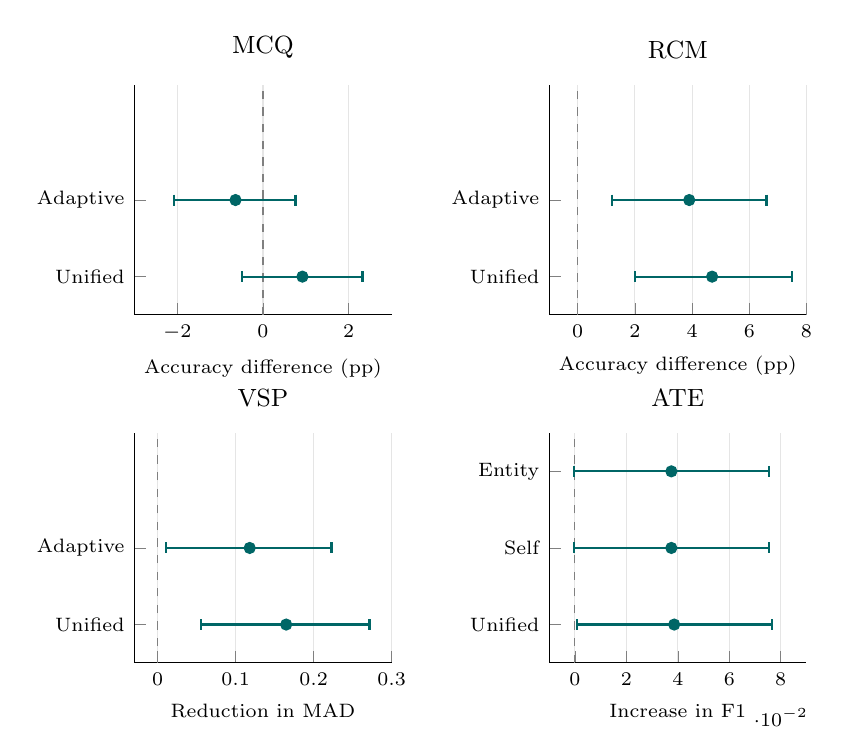
\begin{tikzpicture}
\begin{groupplot}[
 group style={group size=2 by 2,horizontal sep=2cm,vertical sep=1.5cm},
 width=0.40\textwidth,height=4.5cm,
 ymin=0.5,ymax=3.5,
 ytick={1,2},yticklabels={Unified,Adaptive},
 tick label style={font=\scriptsize},label style={font=\scriptsize},title style={font=\small},
 xmajorgrids=true,grid style={gray!20},axis lines*=left,
]
\nextgroupplot[title={MCQ},xlabel={Accuracy difference (pp)},xmin=-3,xmax=3]
\addplot[gray,dashed,forget plot] coordinates {(0,0.5) (0,3.5)};
\addplot[teal!80!black,thick,mark=|] coordinates {(-0.48,1) (2.32,1)};
\addplot[only marks,mark=*,teal!80!black] coordinates {(0.92,1)};
\addplot[teal!80!black,thick,mark=|] coordinates {(-2.08,2) (0.76,2)};
\addplot[only marks,mark=*,teal!80!black] coordinates {(-0.64,2)};
\nextgroupplot[title={RCM},xlabel={Accuracy difference (pp)},xmin=-1,xmax=8]
\addplot[gray,dashed,forget plot] coordinates {(0,0.5) (0,3.5)};
\addplot[teal!80!black,thick,mark=|] coordinates {(2,1) (7.5,1)};
\addplot[only marks,mark=*,teal!80!black] coordinates {(4.7,1)};
\addplot[teal!80!black,thick,mark=|] coordinates {(1.2,2) (6.6,2)};
\addplot[only marks,mark=*,teal!80!black] coordinates {(3.9,2)};
\nextgroupplot[title={VSP},xlabel={Reduction in MAD},xmin=-0.03,xmax=0.3]
\addplot[gray,dashed,forget plot] coordinates {(0,0.5) (0,3.5)};
\addplot[teal!80!black,thick,mark=|] coordinates {(0.0552,1) (0.2717,1)};
\addplot[only marks,mark=*,teal!80!black] coordinates {(0.1648,1)};
\addplot[teal!80!black,thick,mark=|] coordinates {(0.0108,2) (0.2229,2)};
\addplot[only marks,mark=*,teal!80!black] coordinates {(0.118,2)};
\nextgroupplot[title={ATE},xlabel={Increase in F1},xmin=-0.01,xmax=0.09,ytick={1,2,3},yticklabels={Unified,Self,Entity}]
\addplot[gray,dashed,forget plot] coordinates {(0,0.5) (0,3.5)};
\addplot[teal!80!black,thick,mark=|] coordinates {(0.0007,1) (0.0766,1)};
\addplot[only marks,mark=*,teal!80!black] coordinates {(0.0386,1)};
\addplot[teal!80!black,thick,mark=|] coordinates {(-0.0003,2) (0.0753,2)};
\addplot[only marks,mark=*,teal!80!black] coordinates {(0.0375,2)};
\addplot[teal!80!black,thick,mark=|] coordinates {(-0.0003,3) (0.0753,3)};
\addplot[only marks,mark=*,teal!80!black] coordinates {(0.0375,3)};
\end{groupplot}
\end{tikzpicture}
\caption{CTA-RAG effects relative to selected baselines, with pointwise 95\% paired bootstrap intervals. Positive values favor CTA-RAG; the dashed line denotes no difference. Panels have different units and scales. Adaptive denotes Adaptive-RAG-adapted; Self and Entity denote the two tied strongest ATE retrieval baselines. These intervals are not multiplicity-adjusted: an interval excluding zero does not imply rejection after Holm correction across 24 tests (Table~\ref{tab:paired-focus}).}
\label{fig:paired-effects}
\end{figure*}


\paragraph{MCQ: shared retrieval remains competitive.}
Adaptive-RAG-adapted achieves 75.48\% accuracy, compared with 74.84\% for
CTA-RAG, corresponding to a difference of 16 questions. Their paired
comparison does not establish a statistically significant difference after
correction. Nevertheless, every retrieval-based system performs above the
71.00\% Closed Book result. This suggests that supplying relevant factual
evidence captures much of the available MCQ benefit and that specialization
does not provide a demonstrated advantage over the adaptive configuration
for this task.

\paragraph{RCM: exact mapping benefits from task-aligned constraints.}
CTA-RAG reaches 73.40\% accuracy, compared with 68.70\% for Unified RAG
and 69.50\% for Adaptive-RAG-adapted, the strongest competing retrieval
baseline on this task. The RCM specialist combines knowledge-base evidence
with CWE-specific instructions while avoiding the automatic injection of
potentially confusing catalogue neighbours. This design reflects the
task's requirement to identify one primary weakness rather than return a
set of related concepts. The improvement over Unified RAG is statistically
supported, whereas the 3.90-point advantage over Adaptive-RAG-adapted does
not remain significant after Holm correction
($p_{\mathrm{Holm}}=0.0730$).

\paragraph{VSP: task-aligned evidence reduces severity error.}
CTA-RAG obtains a full-attempt MAD of 1.0990, compared with 1.2638 for
Unified RAG and 1.2170 for Adaptive-RAG-adapted. The VSP specialist uses
sanitized historical vulnerability descriptions together with
CVSS-specific instructions to infer the eight base metrics. The baselines
also receive CVSS instructions, so the difference cannot be attributed
to the presence of metric definitions alone. The improvement over Unified
RAG remains significant after correction, while the 0.1180 reduction
relative to Adaptive-RAG-adapted does not
($p_{\mathrm{Holm}}=0.3237$).

On the 992 items successfully completed by every system, CTA-RAG and
Adaptive-RAG-adapted obtain MAD values of 1.0272 and 1.2073,
respectively. This conditional comparison is included only as a sensitivity
analysis because excluding operational failures changes the evaluation
denominator and increases the estimated benefit.

\paragraph{ATE: retrieval provides most of the improvement.}
Unified RAG increases ATE F1 from 0.4149 for Closed Book to 0.9167, while
the other retrieval baselines score between 0.9133 and 0.9178. CTA-RAG
achieves the highest observed F1 of 0.9554, but its smaller advantage over
the retrieval baselines is not statistically established after correction
on the 60-item test set. Technique-focused evidence and output constraints
may contribute to this margin, but the present experiment does not isolate
their causal effect. All saved ATE responses are parseable, indicating that
the large Closed Book deficit primarily reflects incomplete or incorrect
technique sets rather than formatting failures.

Taken together, the results show that the value of specialization is
task-dependent. CTA-RAG provides statistically supported improvements over
Unified RAG on RCM and VSP, where retrieved evidence must be converted into
tightly constrained decisions. Adaptive retrieval remains competitive on
MCQ, while retrieval itself accounts for most of the improvement on ATE.
These findings support task-aligned evidence selection, prompting, and
output constraints, but they do not identify routing as the sole cause
because the specialist indexes, prompts, and pipeline behavior vary
together.

\subsection{RQ2: Can the appropriate specialist be selected automatically?}
\label{sec:robustness}

Under the benchmark instructions used in the controlled evaluation, CTA-RAG
selects the expected specialist for 2,498 of 2,500 MCQ items, 992 of
1,000 RCM items, and every VSP and ATE item. This corresponds to an
overall routing accuracy of 99.78\% (4,550/4,560). The task results are
therefore produced through automatic routing rather than oracle selection,
with only ten routing errors across the complete CTIBench evaluation.

High routing accuracy does not imply high answer accuracy. For example,
RCM routing accuracy is 99.20\%, whereas its final answer accuracy is
73.40\%. Seven of the eight misrouted RCM items result in incorrect
answers, showing that routing errors can propagate to the final prediction.
However, both misrouted MCQ items are answered correctly, indicating that
a routing error does not necessarily produce an incorrect answer. Routing
quality and downstream task performance must therefore be evaluated
separately.

These results establish that the router is reliable for the structured
instructions used in the benchmark. They do not, by themselves, establish
robustness to paraphrased, conversational, underspecified, or content-only
requests. In deployment, the router should detect uncertain task assignments
and request clarification or abstain rather than silently selecting a
potentially inappropriate specialist.


Figure~\ref{fig:route-accuracy} summarizes routing under the current benchmark instructions.
\begin{figure}[t]
\centering
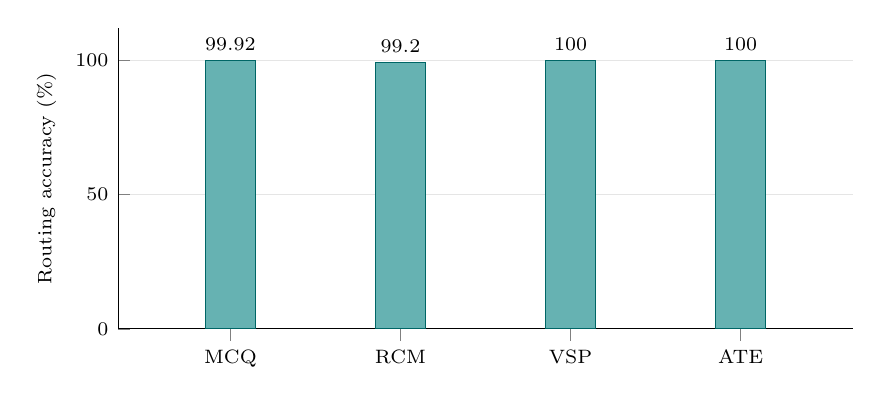
\begin{tikzpicture}
\begin{axis}[
 width=0.90\linewidth,height=5.4cm,
 ybar,bar width=18pt,
 symbolic x coords={MCQ,RCM,VSP,ATE},xtick=data,
 ymin=0,ymax=112,ylabel={Routing accuracy (\%)},
 enlarge x limits=0.22,
 tick label style={font=\scriptsize},label style={font=\scriptsize},
 ymajorgrids=true,grid style={gray!20},axis lines*=left,
 nodes near coords,every node near coord/.append style={font=\scriptsize,/pgf/number format/fixed,/pgf/number format/precision=2}
]
\addplot[fill=teal!60,draw=teal!80!black] coordinates {(MCQ,99.92) (RCM,99.20) (VSP,100) (ATE,100)};
\end{axis}
\end{tikzpicture}
\caption{Automatic routing accuracy on the current controlled runs: 2,498/2,500 MCQ, 992/1,000 RCM, 1,000/1,000 VSP, and 60/60 ATE items. Pooled accuracy is 99.78\%. These values measure pipeline selection, not answer correctness or robustness to instruction rewrites.}
\label{fig:route-accuracy}
\end{figure}

\subsection{RQ3: When does retrieval help or hurt?}
\label{sec:ablations}

Aggregate scores do not reveal whether retrieval consistently improves
predictions or whether its gains offset substantial regressions. We therefore
pair each retrieval-based prediction with the corresponding Closed Book
prediction. For MCQ and RCM, an improvement changes an incorrect answer
to a correct one, while a worsening changes a correct answer to an incorrect
one. For VSP, improvement denotes a reduction in item-level absolute error;
for ATE, it denotes an increase in per-item F1. Table~\ref{tab:utility}
reports both directions using the complete task denominators and the primary
failure-handling policy.

\begin{table*}[t]
\centering
\small
\caption{Paired prediction changes relative to Closed Book. MCQ and RCM
improvements and worsenings correspond to rescues and damages. VSP compares
item-level absolute errors, and ATE compares per-item F1. The values describe
end-to-end system effects and do not isolate retrieval from prompting,
routing, or output handling.}
\label{tab:utility}
\setlength{\tabcolsep}{5pt}
\begin{tabular}{@{}llrrrr@{}}
\toprule
Task & System & Improved & Worsened & Unchanged & Net benefit \\
\midrule
MCQ & Unified RAG & 149 & 76  & 2,275 & +73 (+2.92 pp) \\
MCQ & CTA-RAG     & 267 & 171 & 2,062 & +96 (+3.84 pp) \\
RCM & Unified RAG & 38  & 40  & 922   & -2 (-0.20 pp) \\
RCM & CTA-RAG     & 125 & 80  & 795   & +45 (+4.50 pp) \\
VSP & Unified RAG & 391 & 341 & 268   & +0.0664 \\
VSP & CTA-RAG     & 500 & 267 & 233   & +0.2312 \\
ATE & Unified RAG & 54  & 4   & 2     & +0.5018 \\
ATE & CTA-RAG     & 58  & 0   & 2     & +0.5404 \\
\bottomrule
\end{tabular}
\par\smallskip
\footnotesize
For MCQ and RCM, net benefit denotes the number of additional correct
answers and the corresponding change in accuracy. For VSP and ATE, it
denotes the mean reduction in error or increase in F1, rather than the
difference between the improved and worsened item counts.
\end{table*}

Figure~\ref{fig:current-utility} shows the balance of improved and worsened predictions in the current paired analysis.
\begin{figure*}[t]
\centering
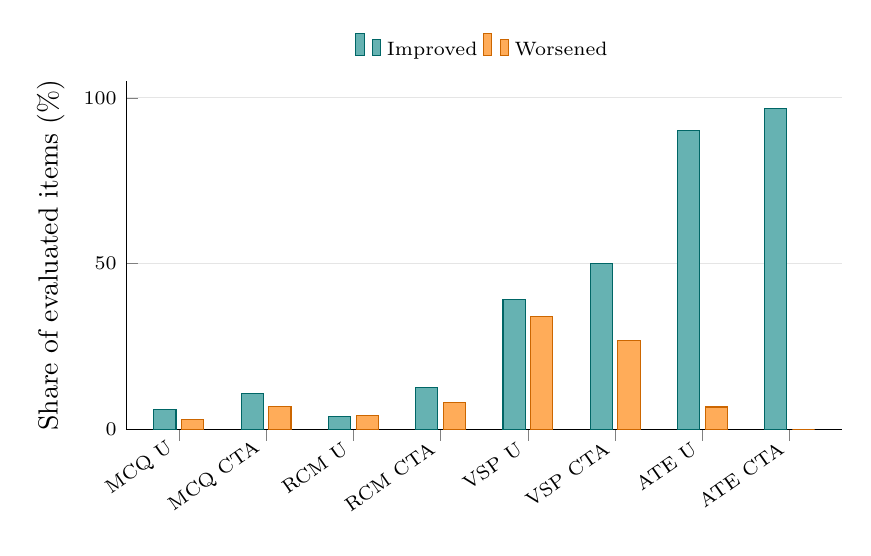
\begin{tikzpicture}
\begin{axis}[
 width=0.88\textwidth,height=6cm,
 ybar,bar width=8pt,
 xmin=0.4,xmax=8.6,ymin=0,ymax=105,
 xtick={1,2,3,4,5,6,7,8},
 xticklabels={MCQ U,MCQ CTA,RCM U,RCM CTA,VSP U,VSP CTA,ATE U,ATE CTA},
 x tick label style={rotate=35,anchor=east,font=\scriptsize},
 yticklabel style={font=\scriptsize},
 ylabel={Share of evaluated items (\%)},
 ymajorgrids=true,grid style={gray!20},axis lines*=left,
 legend style={at={(0.5,1.03)},anchor=south,legend columns=2,draw=none,font=\scriptsize}
]
\addplot[fill=teal!60,draw=teal!80!black] coordinates {(1,5.96) (2,10.68) (3,3.8) (4,12.5) (5,39.1) (6,50) (7,90) (8,96.6667)};
\addplot[fill=orange!65,draw=orange!80!black] coordinates {(1,3.04) (2,6.84) (3,4) (4,8) (5,34.1) (6,26.7) (7,6.6667) (8,0)};
\legend{Improved,Worsened}
\end{axis}
\end{tikzpicture}
\caption{Paired changes relative to Closed Book, expressed as percentages of each task's full denominator. U denotes Unified RAG. Improvement means a newly correct answer for MCQ/RCM, lower error for VSP, or higher item F1 for ATE. Unchanged items are omitted. These are end-to-end system effects; the proportions alone do not measure the magnitude of score changes.}
\label{fig:current-utility}
\end{figure*}


\paragraph{MCQ and RCM show different retrieval behavior.}
Unified RAG rescues 149 MCQ answers while damaging 76, resulting in
73 additional correct answers. CTA-RAG produces a larger net MCQ gain,
with 267 rescues and 171 damages. Both systems therefore benefit from
retrieval on MCQ, although the gains coexist with regressions on individual
questions.

The RCM pattern is substantially different. Unified RAG produces 38 rescues
and 40 damages, resulting in a small net loss of two answers. Retrieval
changes the prediction on many items but provides almost no aggregate
benefit because helpful and harmful changes are approximately balanced.
CTA-RAG produces 125 rescues and 80 damages, yielding 45 additional correct
answers over Closed Book.

A direct comparison between CTA-RAG and Unified RAG shows that CTA-RAG
repairs 124 Unified RAG errors while losing 77 Unified RAG correct answers.
The resulting net improvement of 47 items corresponds to the 4.70-point
accuracy difference reported in Table~\ref{tab:main}. CTA-RAG's advantage
therefore arises from a better balance between helpful and harmful changes,
not from eliminating retrieval-related damage.

\paragraph{VSP and ATE benefit more consistently.}
For VSP, Unified RAG reduces error on 391 items and increases it on 341,
whereas CTA-RAG improves 500 items and worsens 267. The larger CTA-RAG
benefit is therefore distributed across many predictions rather than being
caused by a small number of extreme cases.

Retrieval is most consistently beneficial on ATE. Unified RAG improves
per-item F1 on 54 of 60 items and decreases it on four. CTA-RAG improves
58 items, worsens none, and leaves two unchanged. This pattern is consistent
with the large difference between Closed Book and all retrieval-based ATE
systems: external evidence frequently supplies techniques that the model
does not identify from parametric knowledge alone.

The number of improved and worsened items should not be interpreted as the
metric difference by itself. VSP errors and ATE F1 changes vary in magnitude,
so the average score also depends on how large each item-level change is.

\paragraph{Illustrative prediction changes.}
For the first ATE item, which describes 3PARA RAT, Closed Book predicts the
four reference techniques together with \texttt{T1027} and \texttt{T1552},
producing an F1 of 0.80. Unified RAG and CTA-RAG return the reference set
and obtain an F1 of 1.00. The improvement therefore comes from greater
precision rather than output parseability.

Retrieval can also introduce valid but incorrect identifiers. On RCM item
6, describing local privilege escalation in ZXCLOUD iRAI, Closed Book
matches the reference label \texttt{CWE-269}. Unified RAG instead predicts
\texttt{CWE-78}, while CTA-RAG predicts \texttt{CWE-732}. Both outputs
are syntactically valid but incorrect under the benchmark's exact-label
criterion. These examples illustrate the observed transition categories;
they are not estimates of error prevalence and do not identify which
retrieved passage caused each change.

Overall, retrieval is most consistently useful for ATE and provides a
substantial reduction in VSP error. Its effect is less reliable for exact
CWE mapping: shared retrieval produces nearly equal numbers of RCM rescues
and damages, whereas CTA-RAG shifts this balance toward beneficial changes.
The paired analysis nevertheless measures the complete system, including
retrieval, prompting, routing, and output handling. It therefore demonstrates
when each architecture changes decisions beneficially or harmfully, but
does not attribute those changes to retrieval alone.


\subsection{Threat-actor attribution: candidate recall limits CTA-RAG}\label{sec:taa-results}

The 50-item TAA evaluation is a negative result for the current specialist.
Using the same parser and alias policy for every system, CTA-RAG obtains
25/50 benchmark-compatible matches (50.0\%) and 23/50 strict canonical
matches (46.0\%). TAdaRAG is highest at 36/50, followed by Unified RAG,
Self-Critique RAG, and the local GraphRAG adaptation at 35/50, while
Adaptive-RAG reaches 34/50 and Closed Book 23/50. Thus the specialist
advantage observed on RCM, VSP, and ATE does not extend to attribution.

The saved retrieval traces identify candidate generation as the principal
bottleneck. Among the 12 items solved by TAdaRAG but missed by CTA-RAG, the
gold actor is absent from CTA's internal top-10 pool in nine cases, appears
at ranks 4--10 in two, and is already in the top three in one. A revised
comparison prompt can directly address only the last category; the dominant
failure is that the correct actor is never shown to the generator. We therefore
implemented a provenance-aware graph-inclusion retriever. Its offline 50-item
candidate audit improves dense Recall@1/3/10 from 44/48/60\% to 46/52/68\%,
and MRR@10 from 0.477 to 0.516. This is retrieval-only analysis with no GPT
calls and is exploratory because the same items informed development; it is
not an end-to-end TAA score.

The baseline audit also constrains interpretation. Unified and local GraphRAG
have identical prompt-hash and evidence-size traces on all 50 items and differ
on only one prediction in the earlier TAA reproduction, so that reproduction
is not independent GraphRAG evidence. The corrected ATA GraphRAG-local run is
reported separately below.
Self-Critique RAG is somewhat distinct, but changes only a small subset of
items. The controlled CTA-RAG score therefore remains 25/50, and any
graph-enhanced result must be validated on a new held-out attribution set
before replacing this primary comparison.

\begin{table*}[t]
\centering
\small
\caption{Corrected 50-item CTIBench threat-actor attribution results. All
systems use the same parser and alias normalization; strict identity is a
sensitivity analysis. The local GraphRAG adaptation is reported for
completeness but is not an independent reproduction.}
\label{tab:taa-main}
\begin{tabular}{@{}lcc@{}}
\toprule
System & Benchmark-compatible & Strict identity \\
\midrule
Closed Book & 23/50 (46.0\%) & 22/50 (44.0\%) \\
Unified RAG & 35/50 (70.0\%) & 35/50 (70.0\%) \\
Self-Critique RAG & 35/50 (70.0\%) & 35/50 (70.0\%) \\
GraphRAG (local adaptation) & 37/50 (74.0\%) & 33/50 (66.0\%) \\
Adaptive-RAG-adapted & 34/50 (68.0\%) & 34/50 (68.0\%) \\
TAdaRAG-adapted & \textbf{36/50 (72.0\%)} & \textbf{36/50 (72.0\%)} \\
CTA-RAG & 25/50 (50.0\%) & 23/50 (46.0\%) \\
\bottomrule
\end{tabular}
\end{table*}

\subsection{CTIConnect ATA comparison}\label{sec:ata-results}

The corrected 160-item CTIConnect ATA evaluation uses exact-set accuracy as
the primary metric. Because each item has one gold identifier and the systems
emit one identifier, mean instance F1, precision, recall, and exact-set
accuracy coincide numerically here. The frozen configuration uses hybrid
retrieval with RRF and sends the direct RRF top five candidates to GPT; the
generic MS MARCO reranker is disabled.

\begin{table*}[t]
\centering
\small
\caption{Corrected 160-item CTIConnect ATA results.}
\label{tab:ata-main}
\begin{tabular}{@{}lcccc@{}}
\toprule
System & Exact set / F1 & Precision & Recall & API / parse failures \\
\midrule
Closed Book & 56/160 (35.00\%) & 35.00\% & 35.00\% & 0/0 \\
Unified RAG & 73/160 (45.63\%) & 45.63\% & 45.63\% & 0/0 \\
Self-Critique RAG & 75/160 (46.88\%) & 46.88\% & 46.88\% & 0/0 \\
Adaptive-RAG-adapted & 70/160 (43.75\%) & 43.75\% & 43.75\% & 0/0 \\
TAdaRAG-adapted & 75/160 (46.88\%) & 46.88\% & 46.88\% & 0/0 \\
CTA-RAG & 75/160 (46.88\%) & 46.88\% & 46.88\% & 0/0 \\
GraphRAG-local & \textbf{79/160 (49.38\%)} & 49.38\% & 49.38\% & 0/0 \\
\bottomrule
\end{tabular}
\end{table*}

GraphRAG-local is the strongest ATA result by four items over CTA-RAG, but
the implementation remains a local adaptation rather than a full upstream
GraphRAG reproduction. The ATA result is an end-to-end GPT evaluation; in
contrast, the TAA graph audit is offline and uses no GPT calls.

\subsection{External transfer and operational reliability}\label{sec:transfer}

The completed CTIConnect evaluation covers RCM: every system is evaluated
on the same 290 item IDs and reference mappings. The task's identifier
scorer accepts the dataset's declared alternative targets; with the
single-primary-CWE outputs in these runs, per-item F1 is binary. All items,
including invalid outputs, remain in the denominator. Table~\ref{tab:transfer}
reports the resulting mean F1 and recorded parse validity. No completed
CTIConnect technique-attribution predictions are available, so external
transfer claims here are restricted to RCM.

\begin{table*}[t]
\centering
\small
\caption{Completed external CTIConnect RCM evaluation on 290 shared items. No unresolved API failures remain. Recorded parse validity is shown separately from correctness. The dataset-aware identifier scorer gives binary item F1 for the observed single-CWE predictions.}
\label{tab:transfer}
\setlength{\tabcolsep}{5pt}
\begin{tabular}{@{}lrrr@{}}
\toprule
System & Correct & Mean F1 & Parse validity \\
\midrule
Closed Book & 126/290 & 0.4345 & 67.59\% \\
Unified RAG & 123/290 & 0.4241 & 78.62\% \\
Self-Critique RAG & 124/290 & 0.4276 & 82.07\% \\
Entity-Guided Multi-Query RAG & 110/290 & 0.3793 & 80.00\% \\
Adaptive-RAG-adapted & 123/290 & 0.4241 & 78.62\% \\
Dual-Query RAG & 119/290 & 0.4103 & 77.59\% \\
CTA-RAG & 149/290 & 0.5138 & 97.59\% \\
\bottomrule
\end{tabular}

\end{table*}

Figure~\ref{fig:external-rcm} separates correctness from recorded parse validity on external RCM.
\begin{figure*}[t]
\centering
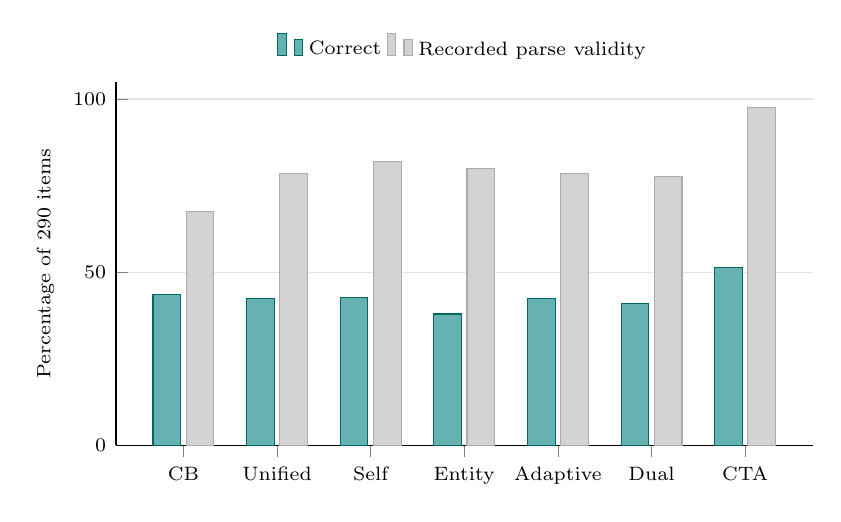
\begin{tikzpicture}
\begin{axis}[
 width=0.86\textwidth,height=6.2cm,
 ybar,bar width=10pt,
 symbolic x coords={CB,Unified,Self,Entity,Adaptive,Dual,CTA},xtick=data,
 ymin=0,ymax=105,ylabel={Percentage of 290 items},enlarge x limits=0.12,
 tick label style={font=\scriptsize},label style={font=\scriptsize},
 ymajorgrids=true,grid style={gray!20},axis lines*=left,
 legend style={at={(0.5,1.03)},anchor=south,legend columns=2,draw=none,font=\scriptsize}
]
\addplot[fill=teal!60,draw=teal!80!black] coordinates {(CB,43.4483) (Unified,42.4138) (Self,42.7586) (Entity,37.9310) (Adaptive,42.4138) (Dual,41.0345) (CTA,51.3793)};
\addplot[fill=gray!35,draw=gray!65] coordinates {(CB,67.59) (Unified,78.62) (Self,82.07) (Entity,80.00) (Adaptive,78.62) (Dual,77.59) (CTA,97.59)};
\legend{Correct,Recorded parse validity}
\end{axis}
\end{tikzpicture}
\caption{External CTIConnect RCM correctness and recorded parse validity on the same 290 items. With the observed single-CWE predictions, mean item F1 equals the fraction correct. Parse validity is a separate diagnostic and does not establish semantic correctness. Abbreviations follow Figure~\ref{fig:current-results}; values come from Table~\ref{tab:transfer}.}
\label{fig:external-rcm}
\end{figure*}


CTA-RAG scores 0.5138, compared with 0.4345 for Closed Book, the strongest
baseline on this dataset, and 0.4241 for Unified RAG. Its improvement over
Closed Book is 23 additional correct mappings, or 7.93 percentage points
(paired 95\% interval: 3.10--12.76 points). Exact McNemar tests
with Holm correction across the six external contrasts support CTA-RAG's
advantage over every baseline (all corrected $p\leq0.0115$).
This is an exploratory external-test family, separate from the 24 main
contrasts. Absolute scores are lower than on CTIBench, and shared retrieval
does not outperform Closed Book here. The findings support an external
RCM advantage, not transfer of the entire four-task pattern or proof that
the external corpus is free of retrieval overlap.

Reliability remains separate from these semantic scores. CTA-RAG produces
valid outputs for all MCQ and ATE items, 930/1,000 CTIBench RCM items,
987/1,000 VSP items, and 283/290 external RCM items. The VSP shortfall
contains five malformed answers and eight unresolved API failures, all
included in the primary penalty-based score. On the external RCM task,
high parse validity coexists with much lower correctness; formatting
alone is not an adequate success criterion.

Recorded CTA invocation-time medians are 6.11, 4.88, 2.31, and 10.74
seconds for MCQ, RCM, VSP, and ATE, respectively. They describe the saved
attempts, not matched end-to-end service latency: CTA timers cover the
pipeline invocation, while baseline timers record the final generation
call, and subsequent format repair is not uniformly included. Internal
token and call accounting is also incomplete for CTA. We therefore provide
the telemetry audit for reproducibility but do not infer cost or latency
superiority from it.

\paragraph{External-transfer and reliability finding.}
The observed CTA-RAG advantage extends to this external weakness-mapping
test, while the other external task remains unevaluated. The results are
consistent with corpus--task alignment mattering, but do not isolate it
causally. Operational success, parse validity, and semantic accuracy must
be reported as distinct outcomes.

\paragraph{Reproducibility.}
We retain item-level predictions, normalized outputs, available run metadata,
prompt versions, model identifiers, corpus-version labels, prediction-file
fingerprints, and analysis seeds. Statistics are recomputed from these fixed
records rather than manually transcribed. Internal CTA metadata are incomplete,
and corpus-version labels do not constitute content fingerprints. API outputs
may vary across model revisions; the paired intervals quantify item-sampling
uncertainty rather than repeated-generation variability.

%%==============================================================================
\section{Operational Implications}\label{sec:impact}
%%==============================================================================

The strongest practical implication is to select a pipeline by the decision
it must support. Shared retrieval is competitive for factual multiple-choice
questions and supplies substantial benefit for technique extraction; weakness
mapping and severity scoring benefit from closer alignment between evidence
and the required answer. The paired analysis also shows that improvements
are accompanied by regressions on other items. An analyst-facing deployment
should therefore evaluate consequential errors, escalation thresholds, and
review burden rather than equating a higher average score with safer triage.
These workflow outcomes were not measured in the benchmark.

Structured outputs make some failures observable and support rejection,
retry, or human review before downstream use. They do not establish semantic
correctness or injection resistance: an incorrect or attacker-influenced
answer can still be a valid CWE or CVSS vector. A practical interface should
request the intended output explicitly, clarify ambiguous requests, and admit
abstention outside the specialist inventory. Complete timing and token
instrumentation is also needed before claiming efficiency benefits. These
controls complement specialization and can be applied to shared RAG systems
as well.

\paragraph{Maintenance Cost of Specialization..}
CTA-RAG shares model-client utilities, embedding interfaces, vector-store
components, and evaluation code, but maintains task-specific retrieval
configurations, prompts, and output handling. Each specialist therefore
requires separate regression coverage, and source updates must be checked
against the pipelines that consume them. Adding a task expands this
configuration and testing surface beyond extending a shared prompt. We did
not measure developer person-hours and claim no quantified maintenance
advantage.

%%==============================================================================
\section{Limitations}\label{sec:limitations}
%%==============================================================================

\paragraph{Benchmark coverage and generalization.}
The main results cover four CTIBench tasks; the external evaluation covers
only CTIConnect RCM. ATE has 60 items, and its additional specialist gain
is not established after multiplicity correction. The paired tests quantify
item-sampling uncertainty for these saved predictions, not model-run
variability. They assume independently sampled evaluation items; shared
reports, related CVEs, or other clustering could make item-level intervals
too narrow. Neither the external result nor template routing accuracy
establishes generalization to unconstrained analyst traffic.
The evaluated datasets, prompts, and routing cues are English, and retrieval
is evaluated in an English-language setting. Dependence on English schema
terms and possible changes in embedding behavior limit multilingual claims.
Translated or native-language CTI benchmarks and language-aware routing and
retrieval are needed to assess that scope.

\paragraph{Baseline fidelity and causal attribution.}
Self-Critique RAG, Entity-Guided Multi-Query RAG, Adaptive-RAG-adapted, and
Dual-Query RAG denote the implemented mechanisms, not full reproductions
of upstream architectures. CTA-RAG differs in prompts, indexes, and pipeline
behavior, so its paired gains do not isolate specialization or retrieval
alone. The task-level mechanisms discussed above are interpretations
supported by the design and diagnostics, not mediation analyses. The
statistical analysis is retrospective rather than preregistered; all
24 primary contrasts are tested and jointly corrected to limit selective
reporting.
The 50-item TAA set was used for post-hoc diagnosis of candidate recall. The
graph-inclusion audit is retrieval-only and exploratory, so it does not replace
the primary end-to-end TAA comparison. The online GraphRAG-local evaluation
obtained 33/50 exact benchmark matches and 37/50 plausible matches. The ATA
table reports the completed corrected 160-item comparison.
The four cognitive modes are an operational decomposition by evidence,
reasoning, and output requirements, not a uniquely necessary taxonomy.
The main comparison does not isolate this grouping against alternatives
based on task identity, knowledge source, output schema, or retrieval
complexity; it therefore cannot establish that the cognitive grouping is
uniquely optimal. The controlled shared-corpus comparison uses dense
retrieval; hybrid BM25--dense retrieval is an orthogonal ablation not
evaluated in the reported main results.

\paragraph{Operational reliability.}
Full-attempt VSP scoring uses an explicit maximum-error penalty for eight
API failures; other service-failure conventions can change the effect size.
The common-success subset is a sensitivity analysis, not a replacement for
the primary denominator. Invalid RCM outputs remain a substantial weakness
of CTA-RAG. Incomplete internal provider, token, and call metadata and
different timing boundaries prevent a controlled efficiency comparison.

\paragraph{Corpus overlap and security.}
Query-time sanitization removes selected leakage signals but does not
establish independence between retrieval corpora and evaluation items,
including the external dataset. Index-level exclusion and overlap audits
would provide stronger evidence. No poisoning or prompt-injection attacks
were evaluated. Task-scoped indexes may limit document exposure when
properly isolated, but neither compartmentalization nor schema validation
should be presented as a measured adversarial defense.
The evaluation also assumes sufficiently reliable indexed sources. The
pipelines do not implement temporal conflict resolution, source-authority
weighting, or cross-source contradiction detection. Task scoping cannot
correct stale or erroneous information within an allowed source, and saved
retrieval provenance is incomplete. Deployment requires source provenance,
snapshot versioning, update monitoring, and abstention or human review when
authoritative sources disagree.

%%==============================================================================
\section{Conclusion}\label{sec:conclusion}
%%==============================================================================

The evaluation shows why task specialization is a useful complement to
retrieval rather than a universal replacement for it. Shared RAG already
provides substantial technique-grounding benefits and remains competitive
on MCQ. CTA-RAG adds statistically supported RCM and VSP gains over Unified
RAG under the full-attempt protocol, while its additional ATE gain and its
differences from the strongest adaptive baseline remain uncertain after
correction. The external RCM evaluation provides further support for the
complete configuration, without establishing four-task transfer.

The answers to the three research questions are therefore connected:
specialization helps selected decision contracts; automatic routing works
well under the tested instructions but remains untested under wording changes; and
retrieval can both rescue and damage individual decisions. The central
design lesson is to align retrieved evidence, instructions, and validation
with the requested decision, and to evaluate that alignment using paired
outcomes and explicit reliability accounting. Isolating the contribution
of each component and validating analyst-workflow benefits remain necessary
steps toward deployment.


\bibliography{references}
\end{document}
